\documentclass[../main.tex]{subfiles}

\begin{document}
\chapter{Liniowo przekształcony rozkład kosinusowy}

Do rozwiązania problemu świateł powierzchniowych można podejść w inny sposób,
autorzy \cite{ltc_heitz} zaproponowali znalezienie przybliżenie wyrażenia
całkowego na sferze następującej postaci:

\begin{displaymath}
I = \int_{P} {
  L(\omega_l)
  \rho(\omega_l, \omega_l)
  \cos \theta_l
  d \omega_l
}
\approx
\int_{P} {
  L(\omega_l)
  D(\omega_l)
  d \omega_l
}
\end{displaymath}

Funkcję $D$ chcielibyśmy dobrać tak, aby całe wyrażenie posiadało wzór jawny
lub było możliwe do przybliżenia w krótkim czasie.

Rozpocznijmy od zdefiniowania warunków, które funkcja $D$ musi spełniać aby
nadawała się do zastosowania jako element przybliżenia. W zaawansowanych
modelach oświetlenia bazowanych na zjawiskach fizycznych występuje kilka
efektów, które muszą zostać zachowane oraz ze względu na różnorodność
materiałów występujących w typowej scenie metoda musi wspierać zmienną
chropowatość powierzchni określoną przez parametr $\alpha$.

Pierwszym z efektów jest odpowiedź funkcji BRDF dla powierzchni obserwowanych
pod odpowiednio dużym kątem. Odpowiedź zostaje rozciągnięta wzdłuż jednej z
osi formując kształt eliptyczny.

Drugim jest to, że w takiej samej sytuacji zwiększając chropowatość materiału
rozkład będzie się rozszerzał i deformował skośnie (ang. \textit{skewness})
powodując, że jest on bardziej rozproszony bliżej normalnej.

Autorzy pracy \cite{ltc_heitz} postanowili najpierw uprościć problem jeszcze
bardziej i znaleźć taki rozkład, który można całkować niezależnie w czasie
rzeczywistym i pozwala modelować powyższe zjawiska. Weźmy dowolny rozkład na
sferze oraz wielokąt  w przestrzeni, który zrzutujemy na sferę. Chcielibyśmy
policzyć całkę:

\begin{displaymath}
\int_P {
  D(\omega)
  d \omega
}
\end{displaymath}

Warto zauważyć, że gdy $D$ jest rozkładem prawdopodobieństwa to powyższa całka
definiuje całkowite prawdpodobieństwo, że próbka wygenerowana z rozkładu $D$
przetnie wielokąt $P$.

Najprostszą, już wcześniej wspomnianą metodą nie nadającą się zbytnio do
zastosowań real-time jest metoda Monte-Carlo wykorzystująca \textit{importance
sampling} polegający na wybraniu losowego wektora z rozkładu $D$ i sprawdzenia
istnienia punktu przecięcia tego promienia z wielokątem. Dla odpowiednio dużej
liczby próbek stosunek trafień do ilości przetestowanych promieni będzie
przybliżał naszą szukaną całkę.

W tym przypadku widać, że rozkład jest równoważny nieskończonej ilości próbek
tego rozkładu, który da się przekształcić z jednego na drugi w sposób
bezpośredni i bezstratny. Zatem rozkład na sferze jest obiektem dualnym do
nieskończonego zbioru ilości próbek tego samego rozkładu \cite{ltc_heitz}.
Wynika z tego to, że po zmodyfikowaniu jednego otrzymamy nowy obiekt
matematyczny.

Przykładem takiej operacji może być przekształcenie liniowe modyfikujące
kierunek próbki (zakładać będziemy, że próbka po przekształceniu liniowym w
dalszym ciągu jest jednostkowej długości tzn. zawsze zostaje z powrotem
znormalizowana). Takie przekształcenie ma kilka bardzo ważnych właściwości
które będziemy wykorzystywać. Warto zauważyć, że jeżeli przekształcimy rozkład
prawdopodobieństwa przekształceniem $M$ to jeżeli zrobimy to samo z wielokątem
$P$ otrzymując wielokąt $P'$, to prawdopodobieństwo, że nowa próbka przetnie
nowy wielokąt się nie zmieni – widać to wyraźnie z faktu, że przekształcone
próbki podążają za przekształcanym wielokątem. Wynika stąd, że:

$$
\int_P {
  D(\omega)
  d \omega
} = \int_{P'} {
  D'(\omega)
  d\omega
}
$$

Rozumowanie można przeprowadzić na odwrót dla macierzy $M^{-1}$. Wynika z tego,
że jeżeli będziemy w stanie znaleźć prosty rozkład bazowy, którego całkę tej
postaci możemy szybko obliczyć oraz przekształcenie $M^{-1}$ przybliżające
rozkład docelowy rozkładem bazowym, to wykorzystując powyższą właściwość możemy
przybliżyć wartość całki rozkładu docelowego na wielokącie sferzycznym.

\begin{figure}[ht]
\missingfigure{Obrazek kilku przekształceń rozkładu LTC}
\end{figure}

Kolejnym zadaniem jest wybór rozkładu bazowego, który po przekształceniu
liniowym da nam oczekiwany rozkład spełniający założenia postawione na
samym początku.

Rozpocznijmy poszukiwania od najprostszego rozwiązywalnego rozkładu, a
mianowicie rozkładu jednorodnego. Jeżeli rozkład $D$ przyjmuje taką samą
wartość w każdym punkcie to całka na wielokącie sferycznym (ang.
\textit{spherical polygon}) jest równoważna kątowi bryłowemu (ang.
\textit{solid angle}) przemnożonym przez odpowiedni stały współczynnik, a na to
istnieje wzór jawny opisany w \cite{Arvo} \cite{Snyder} (Girard's theorem).
Bardzo podobnie sytuacja wygląda z półsferą, z tym że wielokąt musi zostać
przycięty do horyzontu. Rozkład jednorodny opisany na półsferze możemy opisać
wzorem:

$$
D_0(\omega_o=(x_0, y_0, z_0)) = \begin{cases}
  \frac{1}{2\pi} & \text{dla } y_0 \geq 0 \\
  0 & \text{dla } y_0 < 0
\end{cases}
$$

Niestety, oba rozkłady nie są w stanie modelować żadnych ciekawych zjawisk
ze względu na niezmienną naturę.

Nieco bardziej skomplikowanym rozkładem jest przycięty rozkład kosinusowy (ang.
\textit{diffuse}, \textit{Lambertian distribution}, \textit{cosine
distribution}).

$$
D_0(\omega_o=(x_0, y_0, z_0)) = \begin{cases}
  \frac{y_0}{\pi} & \text{dla } y_0 \geq 0 \\
  0 & \text{dla } y_0 < 0
\end{cases}
$$

Zaletą tego rozkładu jest fakt, że przechodzi on gładko do 0 oraz posiada
prosty wzór jawny. Obliczanie całki na takim rozkładzie jest z definicji
obliczaniem irradiancji wielokąta sferycznego. Istnieje wzór jawny
wyprowadzony przez Lamberta \cite{Baum}:

$$
E(p_1, \ldots, p_n) =
\frac{1}{2\pi}
\sum_{i=0}^{n} {
  \cos^{-1}(\langle p_i, p_j \rangle)
  \left\langle {
    \frac{\langle p_i, p_j \rangle}{||\langle p_i, p_j \rangle||},
    \left[ \begin{matrix} 0 \\ 0 \\ 1 \end{matrix} \right]
  } \right\rangle
}
$$

$$
j = (i+1) \text{ mod } n
$$

Złożoność powyższego wzoru jest liniowo zależna od stopnia złożoności
wielokąta, co umożliwia zastosowanie go w aplikacjach czasu rzeczywistego.

Warto również zauważyć, że wszystkie powyższe rozkłady podstawowe mają
postać znormalizowaną tzn. zachodzi warunek:

$$
\int_\Omega {
  D_0(\omega_0)
  d \omega_0
} = 1
$$

Istnieją również inne potencjalne rozkłady bazowe, ale niestety
w większości przypadków nie nadają się one do tego zastosowania. Rozkłady
opisywane przez \textit{spherical gaussian} nie posiadają wzoru jawnego, rozkład
Phong’a posiada wzór jawny, jednak zmienna złożoność zależna liniowo od
wykładnika sprawia, że metoda jest niepraktyczna.

\todo[inline]{Dodatkowo z natury rozkład Phong’a w postaci
nieprzetransformowanej nie modeluje poprawnie zachowań światła przy dużym kącie
padania wiązki światła.}

Z powyższych rozważań, wynika, że przycięty rozkład cosinusowy jest dobrym
kandydatem na rozkład bazowy – gładko przechodzi do 0 oraz posiada prosty
wzór jawny.

Pozostaje wybór przekształcenia liniowego, którego będziemy używać do
formowania naszego przybliżenia. Dla materiału izotropowego funkcja BRDF
zależy tylko i wyłącznie od kąta obserwacji, zatem wektora
  $V = (\sin\theta, \cos\theta, 0)$
oraz współczynnika chropowatości $\alpha$.

Wróćmy znów do efektów które chcemy wymodelować.

Pierwszym, najprostszym z nich jest kontrola chropowatości za pomocą
współczynnika $\alpha$, która może zostać zrealizowana poprzez skalowanie
niejednorodne próbek:

$$
M_{\alpha} =
\begin{bmatrix}
  \lambda & 0 & 0 \\
  0 & \lambda & 0 \\
  0 & 0 & 1
\end{bmatrix}
$$

\begin{figure}[ht]
  \centering
  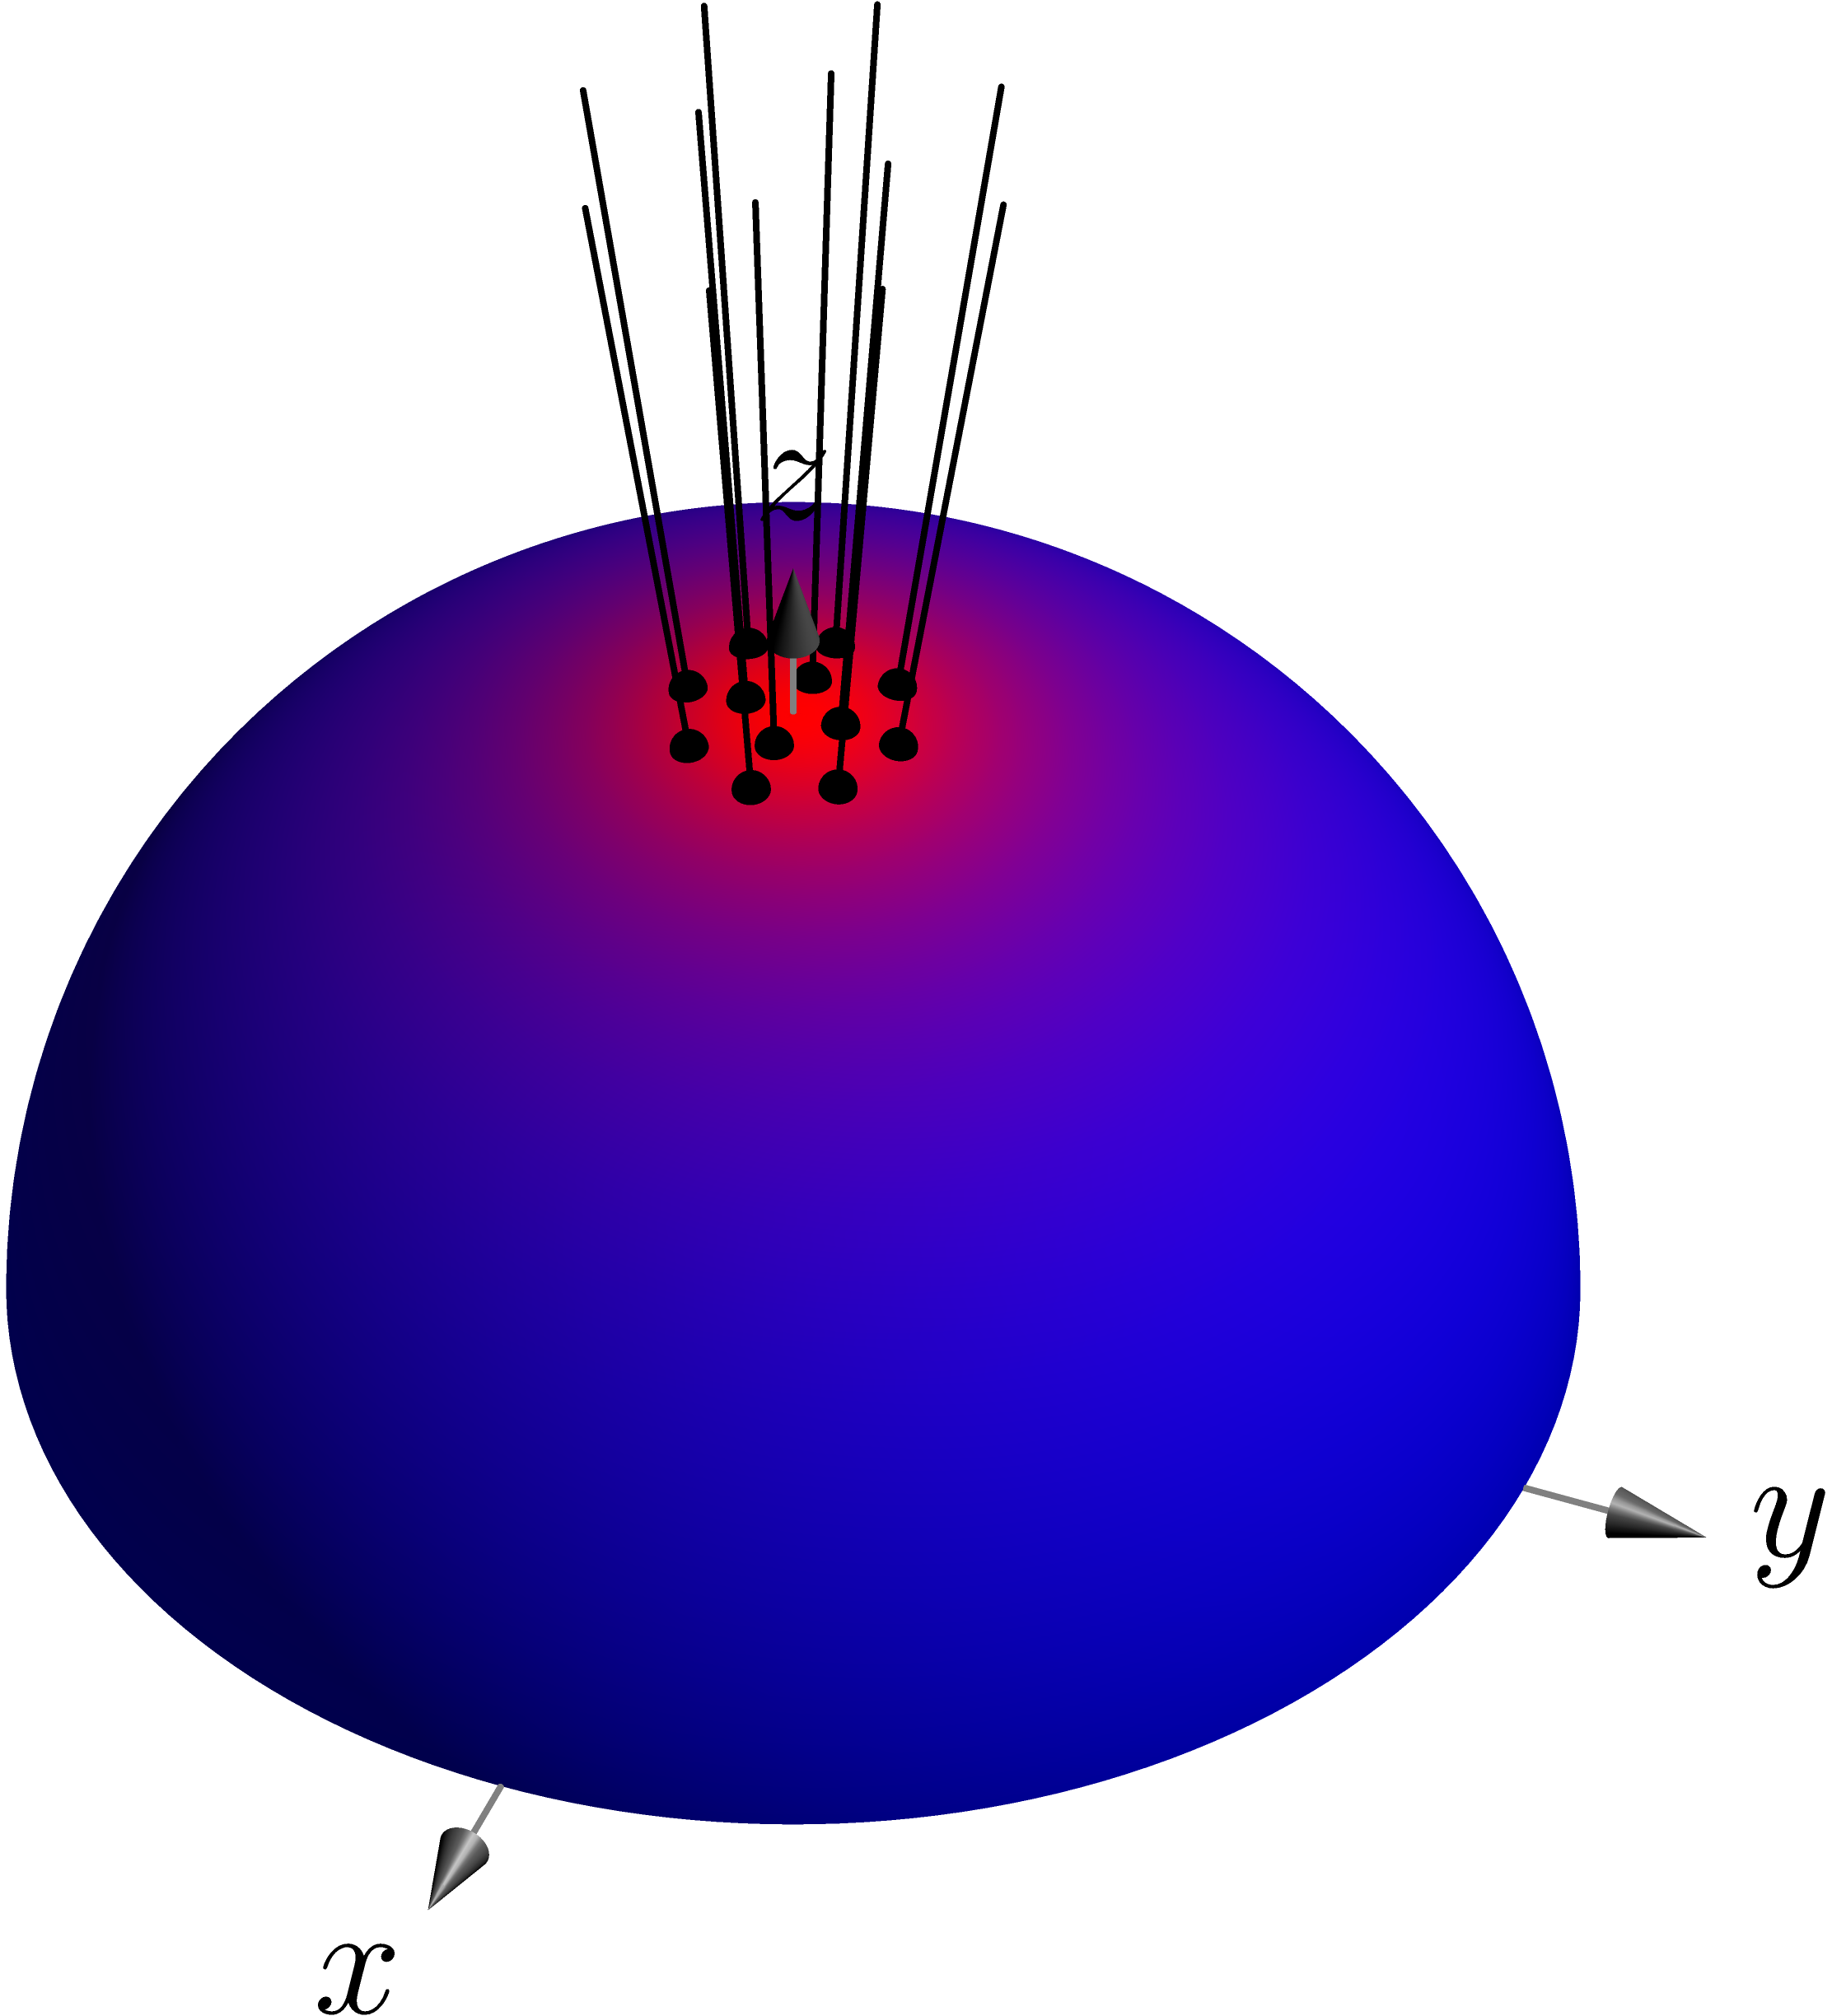
\includegraphics[height=5cm]{ltc/cosine_dist_scale.png}
  \caption{Skalowanie na płaszczyźnie XY.}
  \label{fig:LTCEqualScale}
\end{figure}

Anizotropia:

$$
M_{\text{aniso}} =
\begin{bmatrix}
  \lambda_x & 0 & 0 \\
  0 & \lambda_y & 0 \\
  0 & 0 & 1
\end{bmatrix}
$$

\begin{figure}[ht]
  \centering
  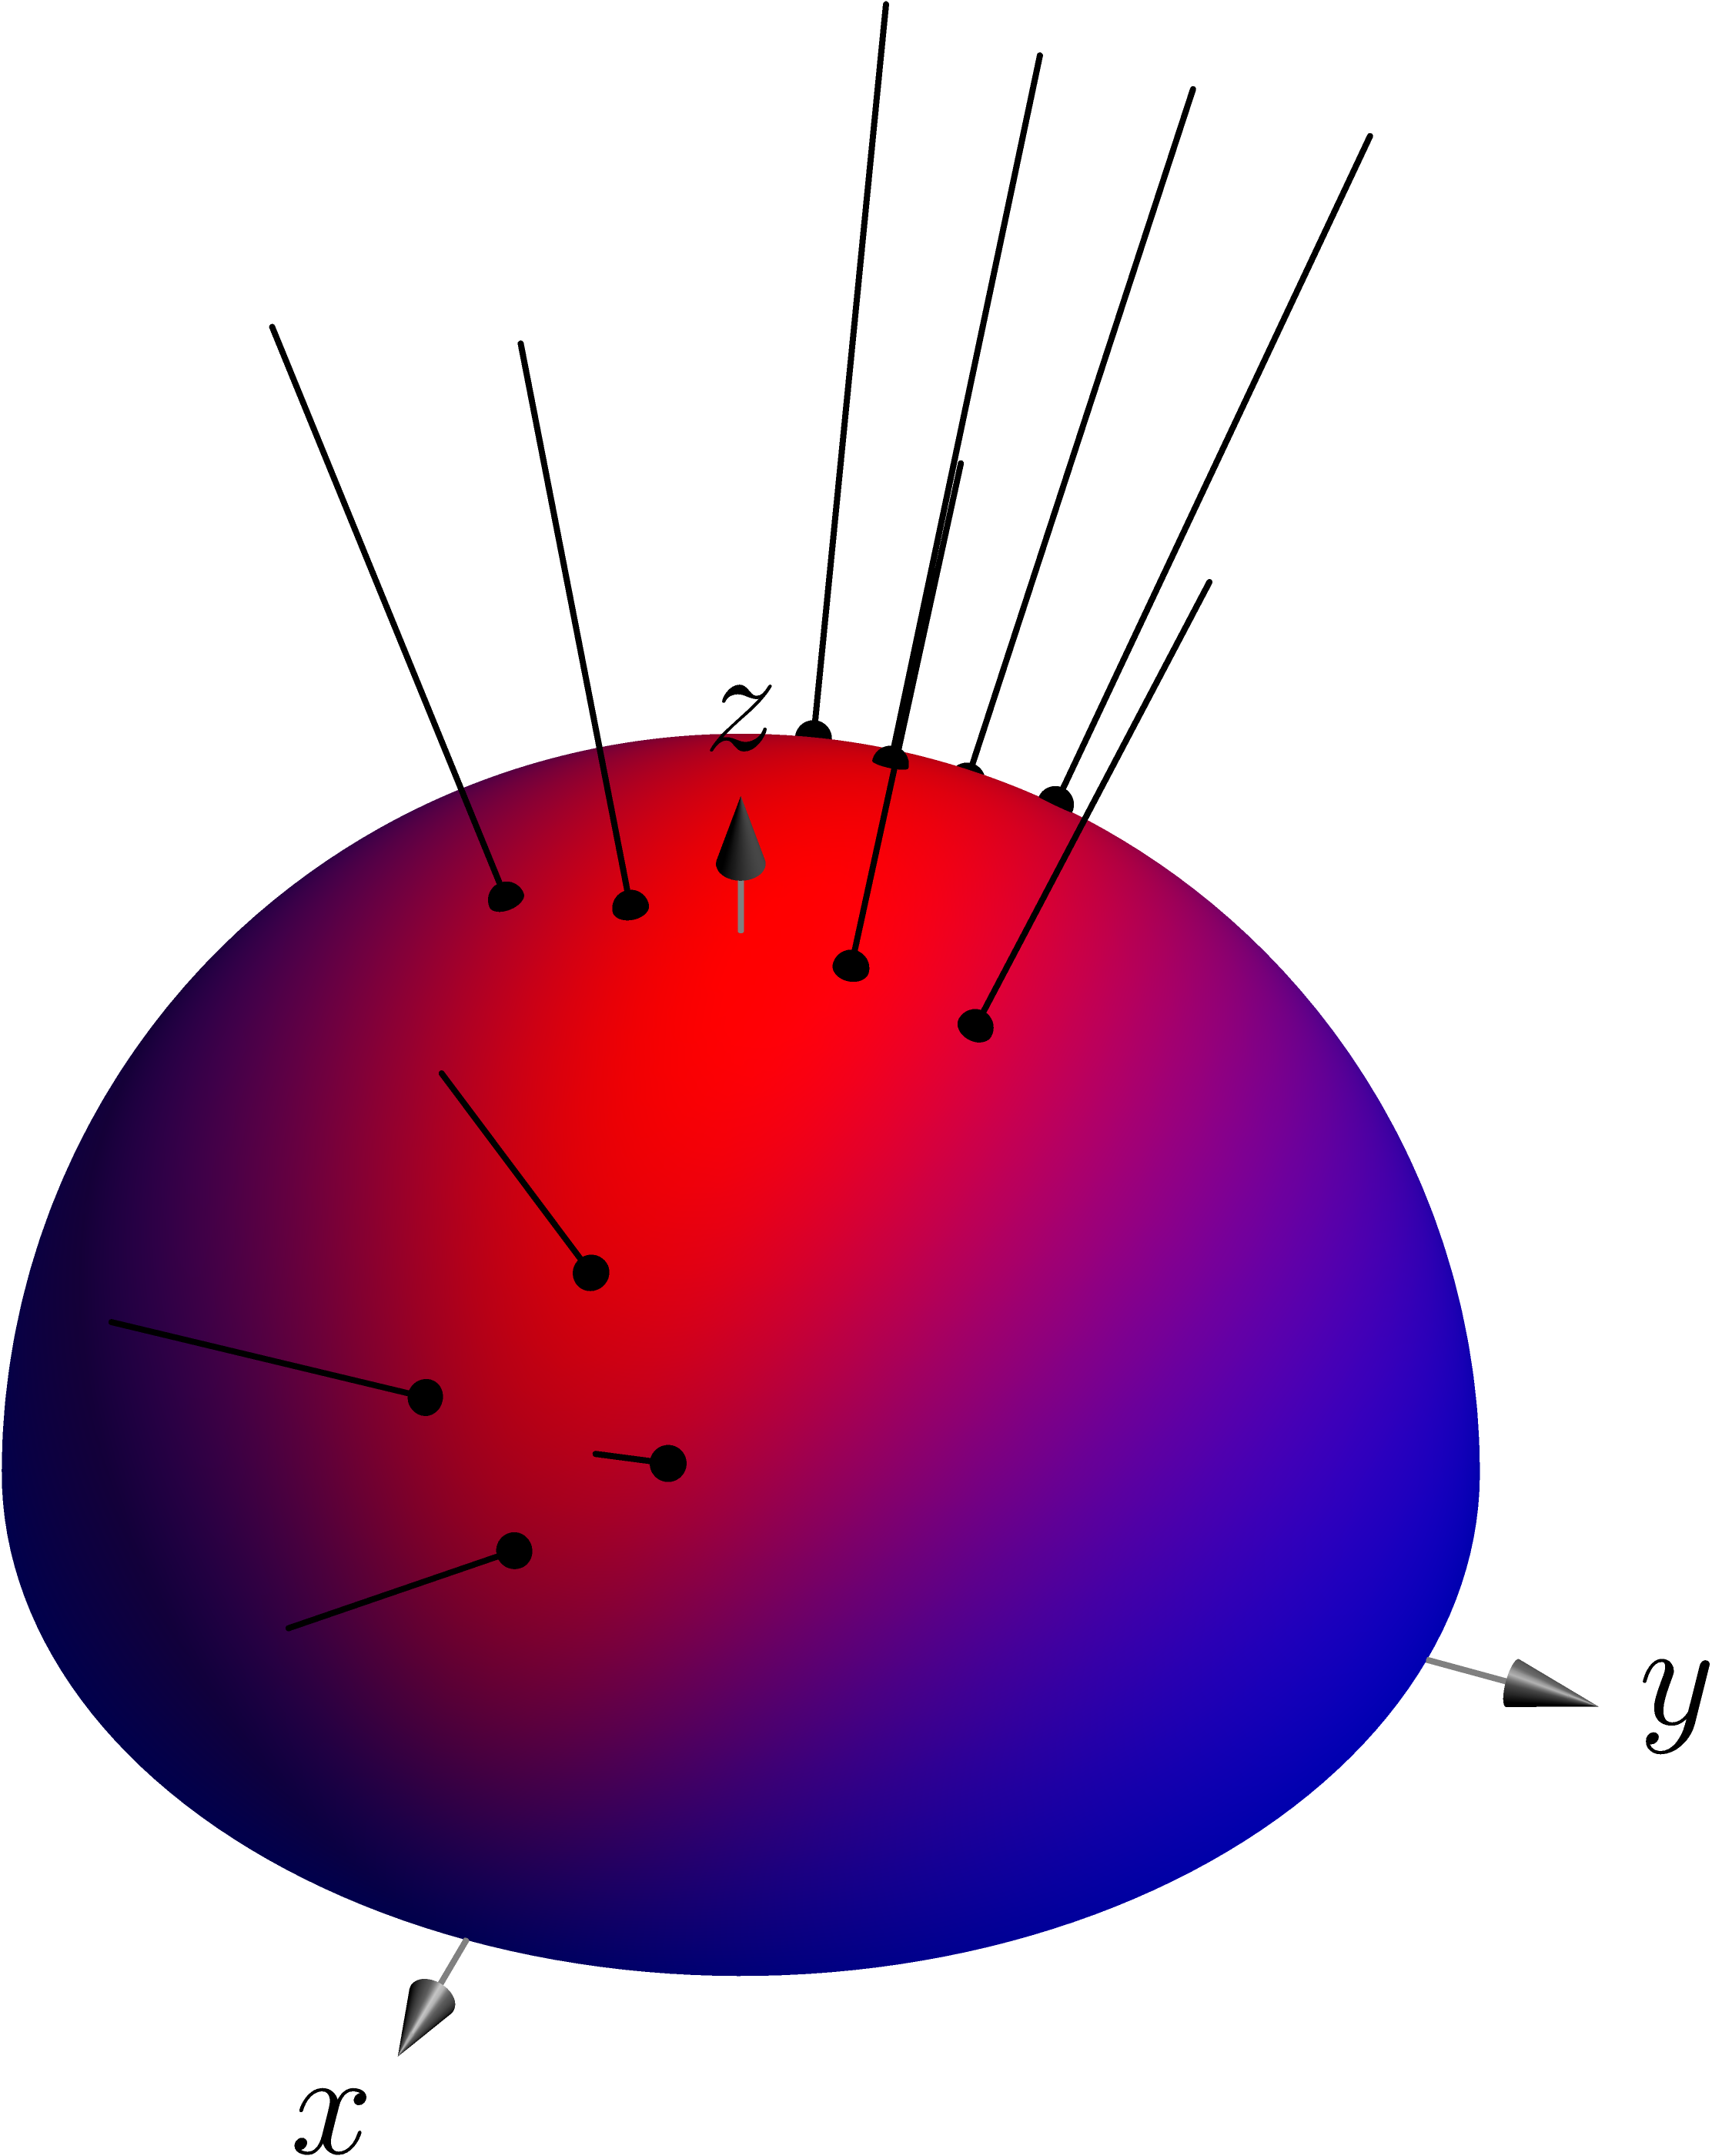
\includegraphics[height=5cm]{ltc/cosine_dist_scale_aniso.png}
  \caption{Skalowanie anizotropowe na płaszczyźnie XY.}
  \label{fig:LTCAnisoScale}
\end{figure}

Skośność przy dużych kątach obserwacji:

$$
M_{\text{skew}} =
\begin{bmatrix}
  1 & 0 & 0 \\
  0 & 1 & 0 \\
  \lambda_{s} & 0 & 1
\end{bmatrix}
$$

\begin{figure}[ht]
  \centering
  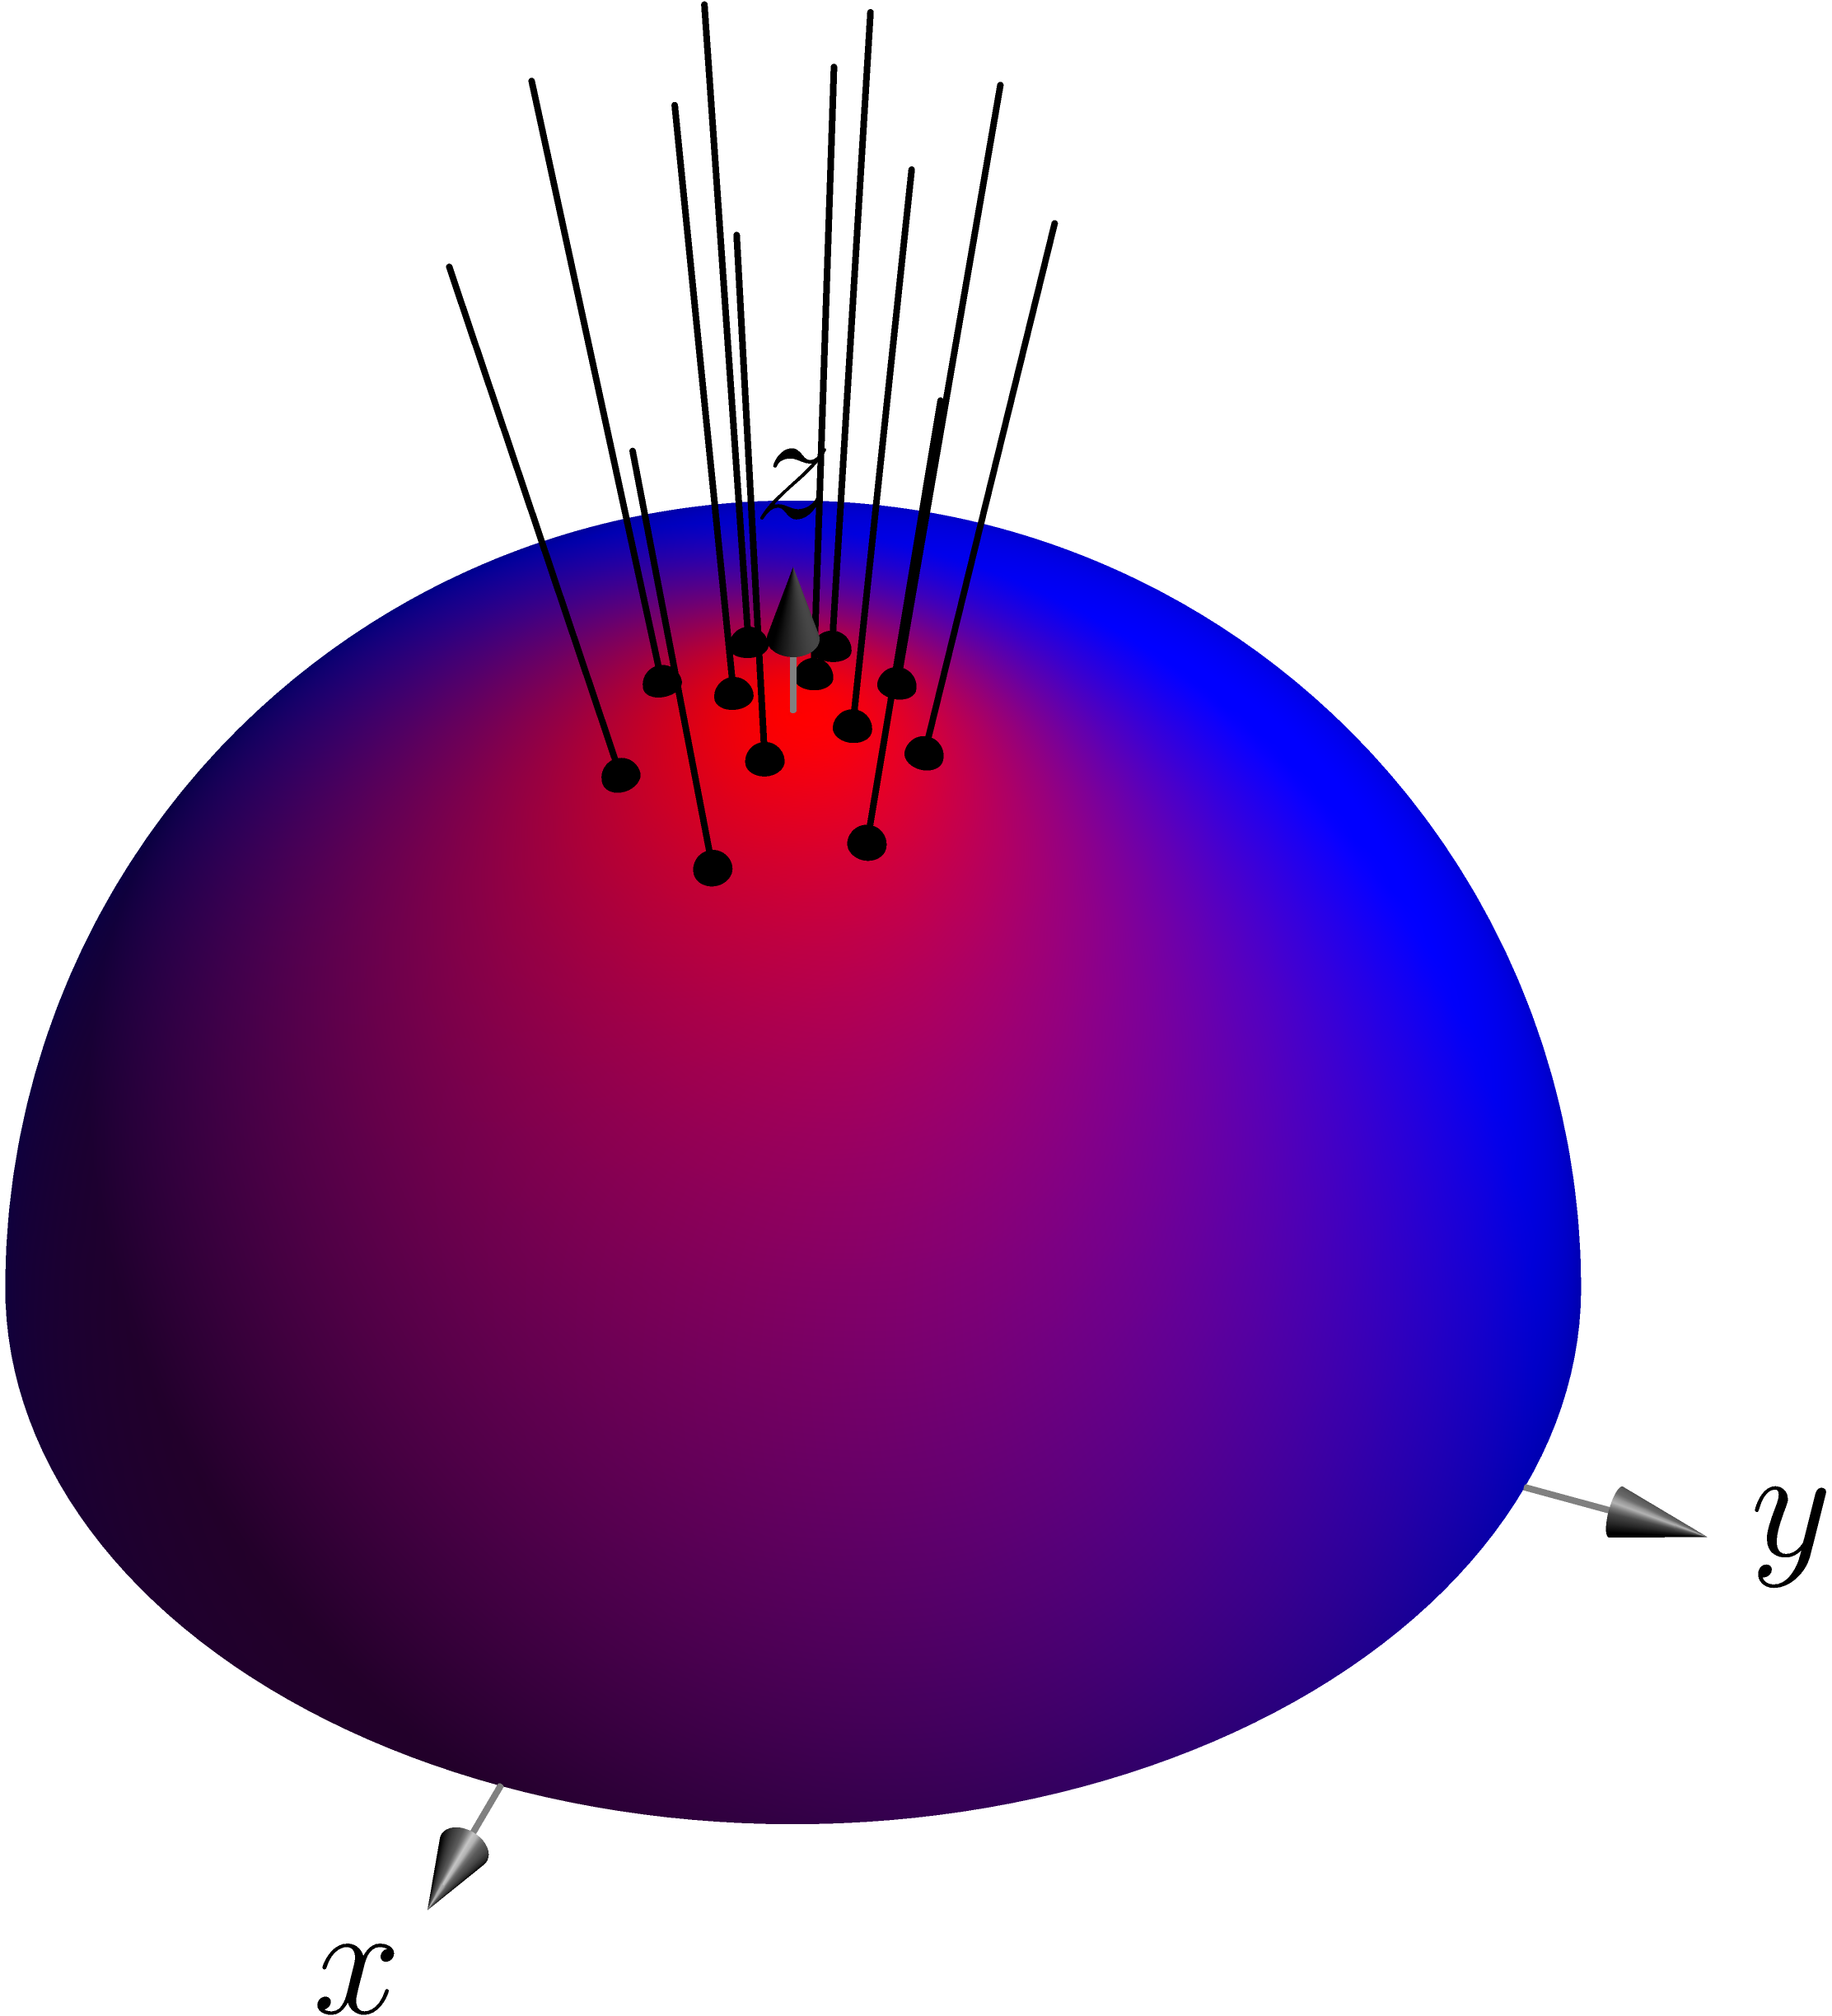
\includegraphics[height=5cm]{ltc/cosine_dist_skew.png}
  \caption{Skośność}
  \label{fig:LTCSkew}
\end{figure}

Widać zatem, że przekształcenie liniowe daje nam możliwość precyzyjnego
modelowania spójnych rozkładów o prostych, ale wystarczających dla naszych
zastosowań kształtach.

Powyższe przekształcenia dają nam możliwość precyzyjnego modelowania
spójnych rozkładów o prostych, ale wystarczających do naszych zastosowań
kształtach. Chcielibśmy teraz znaleźć przekształcenie dla danego kąta
i współczynnika $\alpha$, tak, aby w rezultacie dostać przybliżenie
fizycznie poprawnego rozkładu, np. rozkładu GTR (Generalized
Torrance-Reitz).

Wykorzystamy technikę dopasowywania danych (fitting) przeprowadzoną
\textit{offline} i wykorzystamy gotowe rezultaty podczas rysowania sceny.

Poszukiwaną macierzą przekształcającą jest (dokładne wyjaśnienie dlaczego
wystarczy dalej):

$$
M =
\begin{bmatrix}
  m_{11} & 0 & m_{13} \\
  0 & m_{22} & 0 \\
  m_{31} & 0 & m_{33}
\end{bmatrix}
$$

Dokument \cite{ltc_heitz} sugeruje znormalizowanie macierzy tak aby $m_{33}=1$,
ale powoduje to problemy z interpolacją między poszczególnymi przekształceniami
w stanach pośrednich, w prezentacji \cite{LTCJourneyPresentation} można znaleźć
wyjaśnienie i przykłady problemów niesionych przez te rozwiązanie.

\section{Dopasowywanie rozkładu}

W celu dopasowania przekształcenia liniowego dla danych $\alpha$
i $\theta$ wykorzystamy algorytm pływającego sympleksu \cite{NelderMead65}.

W celu przyśpieszenia dopasowywania znajdziemy najpierw kierunek dominujący
  $\omega_d = \left(sin\theta, 0, \cos\theta\right)$
oraz normę $A$ przybliżanego rozkładu rozkładu. Dane te umożliwią nam wstępne
ustawienie rozkładu bazowego tak, aby najważniejsze kierunki tych rozkładów
pokryły się. Informacje te są możliwe do wyprowadzenia korzystając z metody
Monte Carlo z importance samplingiem, opisanym przez poniższe równania:

$$
A = \int_{\Omega} D_{\text{BRDF}}(\omega)d\omega
\stackrel{n \rightarrow \infty}{=}
\frac{1}{n} \sum_{i=1}^{n} {
  \frac{
    D_{\text{BRDF}}(\omega_i)
  }{
    \text{pdf}_{\text{BRDF}}(\omega_i)
  }
}
$$

$$
\omega_d
\stackrel{n \rightarrow \infty}{=}
\frac{1}{n} \sum_{i=1}^{n} {
  \frac{
    D_{\text{BRDF}}(\omega_i)
  }{
    \text{pdf}_{\text{BRDF}}(\omega_i)
  }
  \omega_i
}
$$

W przypadku anizotropowym chcielibyśmy przeprowadzać obliczenia w pewnej
płaszczyźnie ze względu na uproszczenie obliczeń, w naszym przypadku
założyliśmy że $Y=0$ dla kierunku obserwacji. \todo{Wyjaśnić dokładniej.}
Obliczenie kierunku $\omega_d$ metodą Monte-Carlo może spowodować zajście
warunku $Y \neq 0$. Dlatego też dokonujemy "przyciągnięcia" wektora do
osi:

$$
\widetilde{\omega}_d = \frac{
    \left( \omega_x,0,\omega_z \right)
  }{
    w_x^2+w_z^2
  }
$$

Kolejnym krokiem jest ustawienie "czubka" rozkładu kosinusowego w kierunku
dominującym $\omega_d$, czyli zbudowanie układu w którym oś $Z$ będzie
pokrywać się z kierunkiem $\omega_d$. Uzyskana macierz $M_{\text{rot}}$
będzie częścią składową finalnej macierzy $M$.

$$
M_{\text{rot}} =
\begin{bmatrix}
  \cos\theta  & 0     & \sin\theta \\
  0           & 1     & 0 \\
  -\sin\theta & 0     & \cos\theta
\end{bmatrix}
= \begin{bmatrix}
  \bot {\widetilde{\omega}_d} & Y & \widetilde{\omega}_d
\end{bmatrix}
$$

Kolejnym krokiem jest ukształtowanie rozkładu do formy uwzględniającej
faktyczną odpowiedź tj. chropowatość ($\alpha$), anizotropowość przy
dużych kątach obserwacji i efekt skośny (występujący na jednej z osi):

$$
M_{\text{precise}} =
\begin{bmatrix}
  1 & 0 & \lambda_{\text{skew}} \\
  0 & 1 & 0 \\
  0 & 0 & 1
\end{bmatrix}
\begin{bmatrix}
  \lambda_x & 0 & 0 \\
  0 & \lambda_y & 0 \\
  0 & 0 & 1
\end{bmatrix}
\begin{bmatrix}
  \lambda & 0 & 0 \\
  0 & \lambda & 0 \\
  0 & 0 & 1
\end{bmatrix}
=
\begin{bmatrix}
  \lambda\lambda_x & 0 & \lambda_{\text{skew}} \\
  0 & \lambda\lambda_y & 0 \\
  0 & 0 & 1
\end{bmatrix}
\stackrel{\text{ozn.}}{=}
\begin{bmatrix}
  a & 0 & c \\
  0 & b & 0 \\
  0 & 0 & 1
\end{bmatrix}
$$

Zatem finalna macierz $M$ ma postać:

$$
M = M_{\text{rot}} M_{\text{precise}}
$$

w której prawdziwymi niewiadomymi są tylko trzy zmienne $a$, $b$ i $c$.

Macierz $M$ ze specyfiki metody musi być odwracalna, zatem:
  $\det M \neq 0 \Rightarrow ab \neq 0$.
Wprowadzimy dodatkowe założenie, że parametry $a$ i $b$ są dodatnie, ze względu
na to, że ujemny parametr będzie oznaczał odbicie lustrzane względem osi.
W ten sposób również zagwarantujemy sobie poprawność znalezionego rozwiązania.

\subsection{Metoda pływającego sympleksu}

Zdefiniujmy nasz problem w postaci problemu optymalizacyjnego. Chcielibyśmy
zminimalizować funkcję $f(a,b,c)$, będącą miarą różnicy (błędu) absolutnej
pomiędzy oryginalnym rozkładem, a przybliżonym. Formalną definicję funkcji
opiszę w kolejnym podrozdziale.

Funkcja ta posiada dwa ograniczenia narzucone przez warunek $detM \neq 0$,
a mianowicie:
  $a > 0 \wedge b > 0$

Oryginalna metoda pływającego sympleksu nie posiada mechanizmu dla ograniczeń,
ale istnieją techniki pozwalające rozwiązać ten problem. W mojej implementacji
wykorzystałem logarytmiczną wewnętrzną (barierową) funkcję kary:

\[
  p_{\mathbb{L}}(x, \rho) = - \frac{1}{\rho} \sum_{i=1}^{m} \log(-g_i(x))
\]

Alternatywną funkcją barierową jest funkcja hiperboliczna:

\[
  p_{\mathbb{H}}(x, \rho) =
    - \frac{1}{\rho} \sum_{i=1}^{m} \frac{1}{g_i(x)}
\]

\subsection{Wyznaczanie błędu przybliżenia}

Mając pewne parametry $a$, $b$, $c$ będące wynikiem kroku algorytmu optymalizacji
chcielibyśmy ocenić jakość przybliżenia wyznaczonego przez te parametry. W tym
celu stworzymy funkcję błędu:

\[
  f(a,b,c) =
    \int_{\Omega} {
      \left| {D_{\text{LTC}}(a, b, c, \omega) - D_{\text{BRDF}}(\omega)} \right|
    } d \omega
\]

Funkcja ta może zostać obliczona z wykorzystaniem techniki MIS opisanej w
rozdziale \ref{Chapter:MIS}.

\subsection{Format danych}

\end{document}
